%\begin{figure}[h]
%	\section{Robot 11} %cambiar titulo
%	\centering
%	{%
%		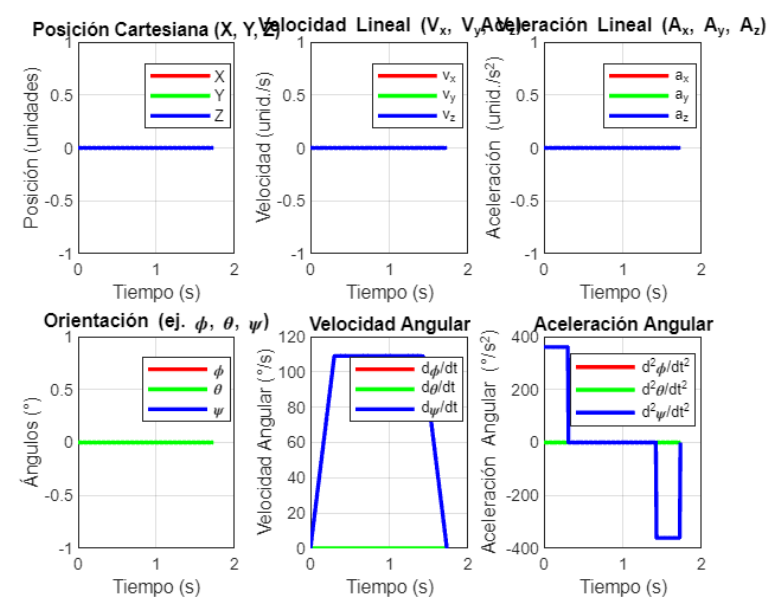
\includegraphics[width=0.8\linewidth]{img/robot11_1}
%		\caption{} %pie de imagen
%		\label{fig:robot11}
%	}
%\end{figure}
%
%\begin{figure}[h]
%	\centering
%	{%
%		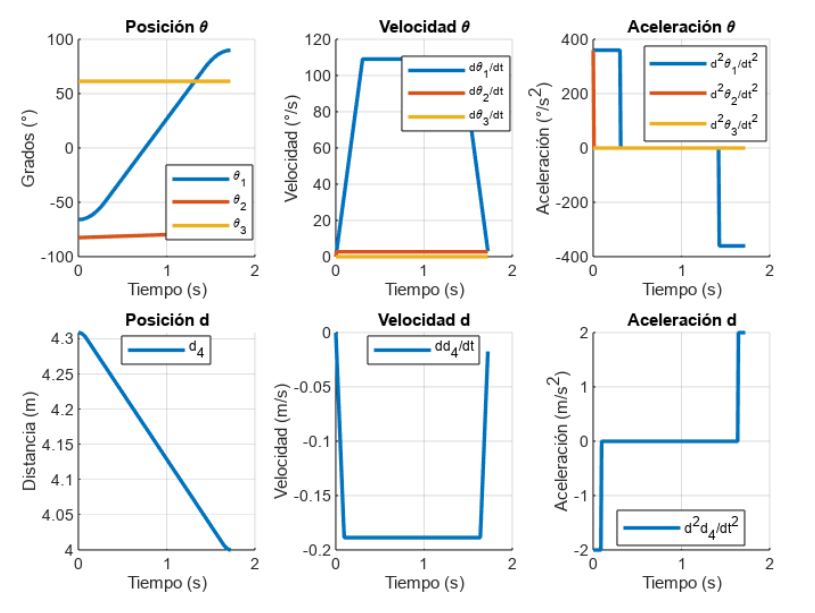
\includegraphics[width=0.8\linewidth]{img/robot11_2}
%		\caption{} %pie de imagen
%		\label{fig:robot_11}
%	}
%\end{figure}
%
%\begin{figure}[h]
%	\centering
%	{%
%		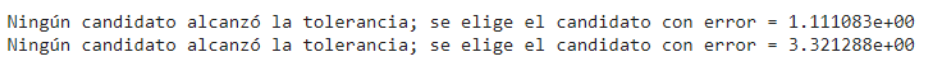
\includegraphics[width=0.8\linewidth]{img/robot11_3}
%		\caption{Error del objetivo} %pie de imagen
%		\label{fig:robot_11_error}
%	}
%\end{figure}

\begin{figure}[h]
	\section{Robot 11} 
	\centering
	\subfloat[]{%
		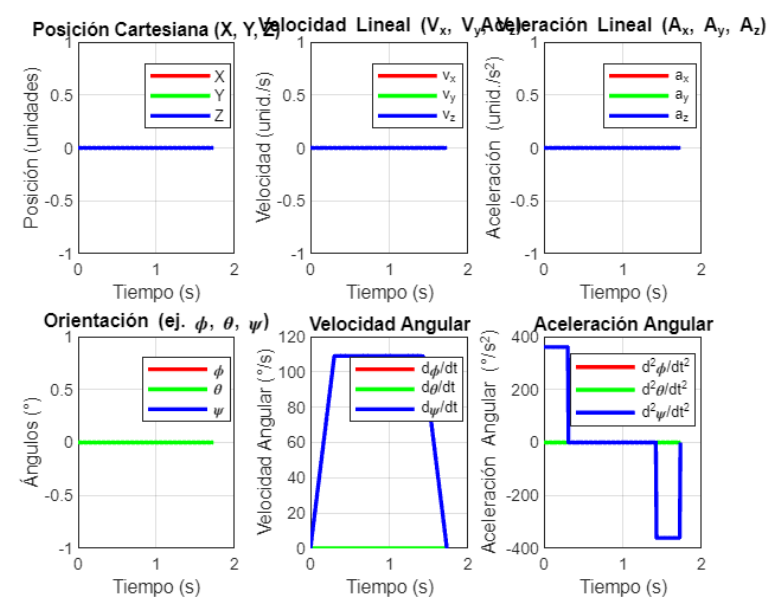
\includegraphics[width=0.75\textwidth]{img/robot11_1}%
		\label{fig:robo11_1}
	}
	\hfill
	\subfloat[]{%
		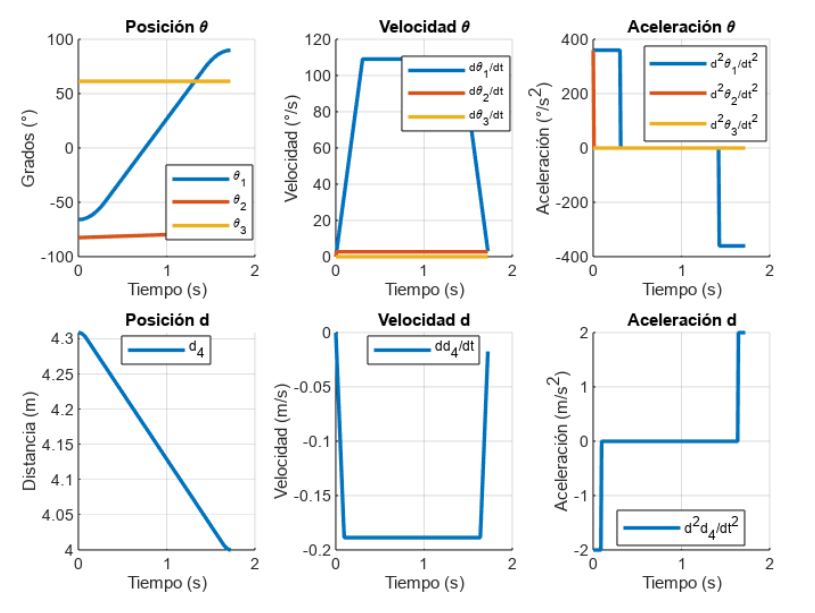
\includegraphics[width=0.75\textwidth]{img/robot11_2}%
		\label{fig:robot11_2}
	}
		\hfill
	\subfloat[Error del objetivo]{%
		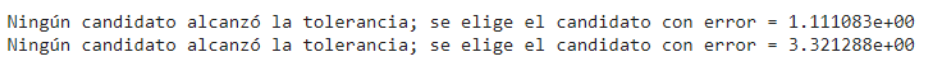
\includegraphics[width=0.8\textwidth]{img/robot11_3}%
		\label{fig:robot11_3}
	}
	\caption{Robot 11}
	\label{fig:Robot11}
\end{figure}